\documentclass[11pt]{article}
\usepackage[utf8]{inputenc}
\usepackage[dvipsnames]{xcolor}
\usepackage{tikz}
\usepackage{enumitem}
\usepackage{hhline}
\topmargin=-0.45in
\evensidemargin=0in
\oddsidemargin=0in
\textwidth=6.5in
\textheight=9.0in
\headsep=0.25in
\begin{document}

\begin{titlepage}
    \begin{center}
        \begin{tikzpicture}[remember picture,overlay]
            \node[anchor=north west,yshift=-1.5pt,xshift=1pt]%
            at (current page.north west)
            {
\includegraphics[scale=1]{ethlogo.pdf}};
        \end{tikzpicture}
        \begin{tikzpicture}[remember picture,overlay]
              \node[anchor=north east,inner sep=0pt, xshift=-0.2cm] at (current page.north east)
              {
\includegraphics[scale=0.4]{systems-logo.pdf}};
        \end{tikzpicture}

            
        \Huge
        \textbf{Cloud computing architecture}
            
        \vspace{0.5cm}
        \LARGE
        Semester project report
            
        \vspace{1.5cm}
            
        \textbf{Group 027}
            
        Jiale Chen - 20-961-504 \\
        Ran Liao - 20-949-186 \\
        Xintian Yuan - 20-951-778 \\
        \vfill
            
            
        \Large
        Systems Group\\
        Department of Computer Science\\
        ETH Zurich\\
        \today
            
    \end{center}
\end{titlepage}
\section*{Instructions}
Please do not modify the template, except for putting your solutions, names and legi-NR.
Parts 1 and 2 should be answered in maximum six pages (including the questions).
\textbf{If you exceed the space, points might be subtracted}.
\newpage
\section*{Part 1 [20 points]}
\begin{enumerate}
            \item \textbf{[10 points]} Plot a single line graph with 95th percentile latency on the y-axis (the
            y-axis should range from 0 to 10 ms) and QPS on the x-axis (the x-axis should range from 0 to 55K).
            Label your axes. State how many runs you averaged across (we recommend three) and include error bars.
            There should be 7 lines in total in your plot, showing the performance of memcached running with no
            interference and six different sources of interference: \texttt{cpu}, \texttt{l1d}, \texttt{l1i}, \texttt{l2}, \texttt{llc}, \texttt{memBW}. The readability of your
            plot will be part of your grade.
            
            \textbf{Solution:} Due to resource contention introduced by the interference, the target QPS cannot be achieved after 25K for \texttt{cpu} and \texttt{l1i} and after 35K for \texttt{llc}, thus the points are overlapped. To ensure readability, we averaged the overlapping points to a single point.
            
            \begin{center}
            {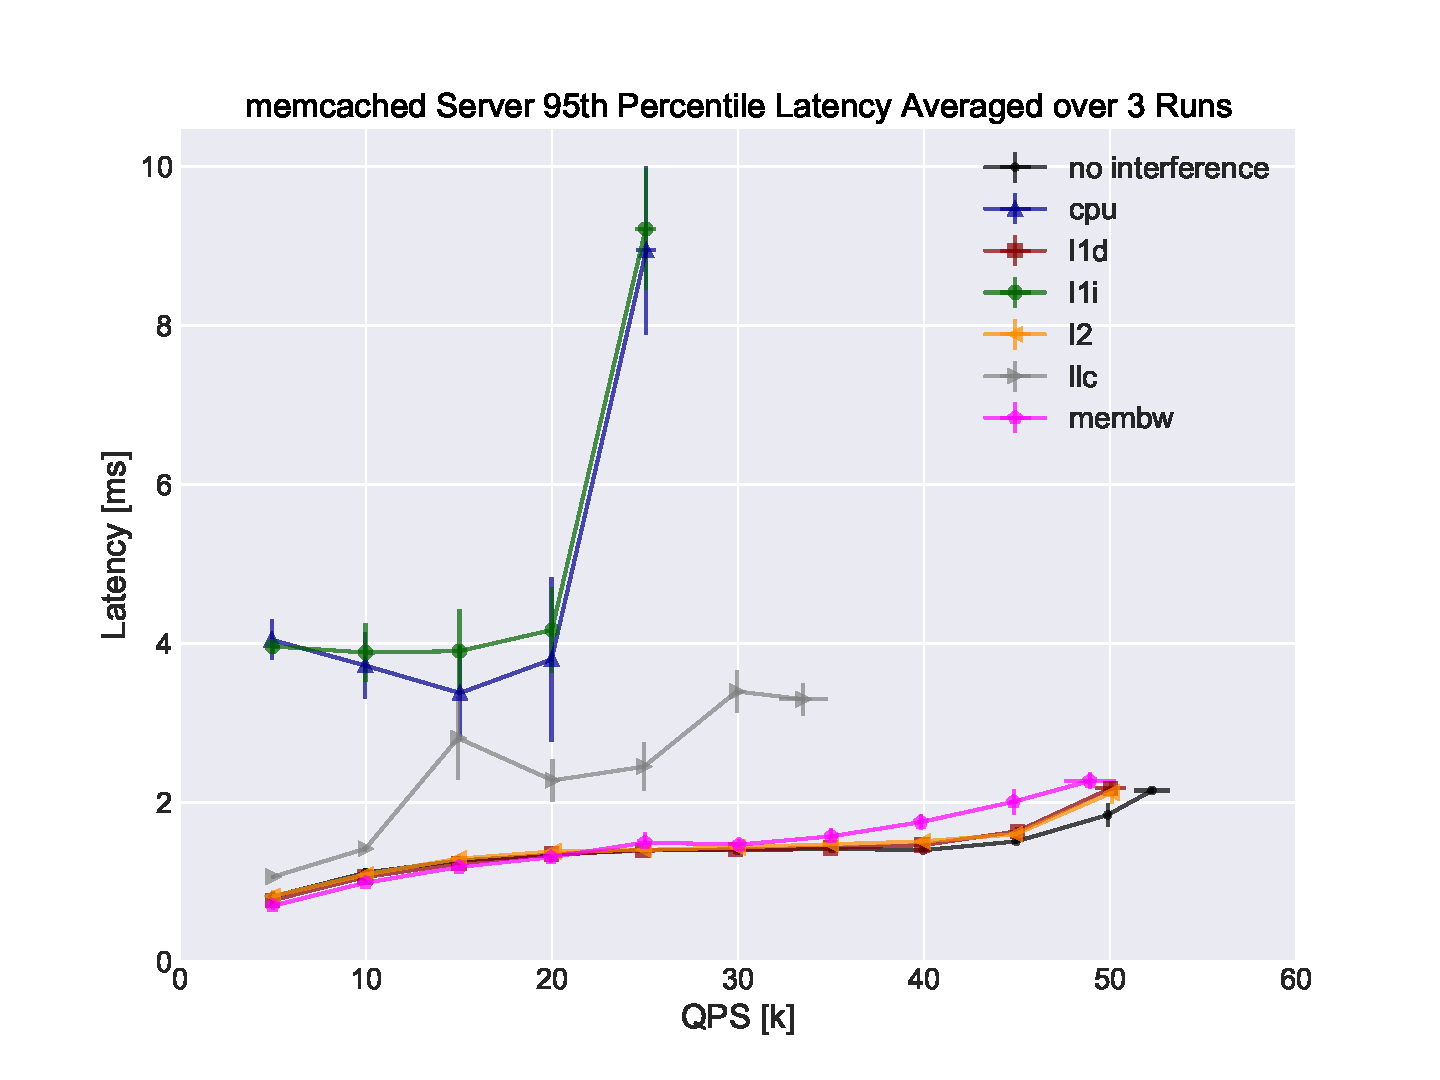
\includegraphics[scale=0.5]{p95.pdf}}
            \end{center}
            
            \item \textbf{[6 points]} Describe how the tail latency and saturation point (the “knee in the curve”) of
            memcached is affected by each type of interference. Also describe your hypothesis for why performance is
            affected in this way.
            
            \textbf{Solution:} The \texttt{l2}, \texttt{l1d} and \texttt{memBW} interference have minor influences on tail latency. Their lines with interference are quite similar to the line without interference. Their saturation points are around 30K QPS. \texttt{llc} interference affects tail latency more significantly when QPS is larger than 10K. \texttt{cpu} and \texttt{l1i} interference increase tail latency significantly from less than 2 ms to more than 4 ms. The saturation point is around 20K QPS. In my opinion, memcached is a CPU intensive job and requires a large amount of CPU resources. Therefore, interference on \texttt{cpu} and \texttt{l1i} cache makes memcached very inefficient. The data accessed in memcached might be quite random and have little locality, thus, tail latency is largely dominated by the speed of moving data between memory and CPU. The cache is somewhat irreverent and has little influence.
            
            \item \textbf{[2 points]} Explain the use of the taskset command in the container commands for memcached and iBench
            in the provided scripts. Why do we run some of the iBench benchmarks on the same core as memcached and others on a different core?
            
            \textbf{Solution:} Each core has its own separate L1 and L2 cache, therefore, interference on such caches must be conducted on the same core. 
            % http://web.cs.wpi.edu/~cs4515/d15/Protected/LecturesNotes_D15/Week3_TeamA_i7-Presentation.pdf page 8
            Since the last level cache and main memory are usually shared across all cores, it's fine to do such interference on a different core. And CPU interference should affect the target core directly.
            
            \item \textbf{[2 point]} Assuming a service level objective (SLO) for memcached of up to 2 ms 95th percentile latency at 40K QPS,
            which iBench source of interference can safely be collocated with memcached without violating this SLO? Explain your reasoning.
            
            \textbf{Solution:} \texttt{l1d}, \texttt{l2}, and \texttt{memBW}. According to the figure in the previous question, only these 3 kinds of interference have minor influence on tail latency, making it less than 2 ms on 40K QPS. Other interference will make memcached unable to reach 40K QPS at all.
            
\end{enumerate}
\section*{Part 2 [25 points]}
\begin{enumerate}
    \item \textbf{[12 points]} Fill in the following table with the normalized execution time of each batch job with each source of
    interference. The execution time should be normalized to the job’s execution time with no interference. Color-code each field in the
    table as follows: {\color{Green}green} if the normalized execution time is less than or equal to 1.3, {\color{YellowOrange}orange} if the normalized execution time is over 1.3
    and up to 2, and {\color{Red}red} if the normalized execution time is greater than 2. Summarize in a paragraph the resource interference sensitivity of
    each batch job.
    
    \textbf{Solution:} The readings are taken from the ``real" time for \texttt{dedup}, \texttt{blackscholes} and \texttt{canneal} as indicated in the logs. For \texttt{ferret}, \texttt{freqmine} and \texttt{fft} benchmarks we used ``QUERY TIME", ``FPgrowth cost" and ``Computation Time" respectively for the calculations. To get the values in the table, we first averaged the readings from three repeated trials, then normalized the ones with interference respect to the normal ones. The results are summarized in the following table.
    
\begin{center}
\begin{tabular}{ |c|c|c|c|c|c|c|c| } 
\hline
 \textbf{Workload} & \texttt{\textbf{none}} & \texttt{\textbf{cpu}} & \texttt{\textbf{l1d}} & \texttt{\textbf{l1i}} & \texttt{\textbf{l2}} & \texttt{\textbf{llc}} & \texttt{\textbf{memBW}}  \\
 \hline\hline
dedup         & 1.0 & \color{YellowOrange}1.52 & \color{Green}1.24 & \color{Red}2.21 & \color{Green}1.24 & \color{Red}2.13 & \color{YellowOrange}1.66 \\  \hline
blackscholes  & 1.0 & \color{YellowOrange}1.42 & \color{YellowOrange}1.42 & \color{YellowOrange}1.89 & \color{YellowOrange}1.38 & \color{YellowOrange}1.73 & \color{YellowOrange}1.45 \\  \hline
ferret        & 1.0 & \color{YellowOrange}1.98 & \color{Green}1.06 & \color{Red}2.77 & \color{Green}1.05 & \color{Red}2.78 & \color{Red}2.20 \\  \hline
freqmine      & 1.0 & \color{Red}2.04 & \color{Green}1.01 & \color{Red}2.06 & \color{Green}1.02 & \color{YellowOrange}1.92 & \color{YellowOrange}1.61 \\  \hline
canneal       & 1.0 & \color{YellowOrange}1.40 & \color{YellowOrange}1.46 & \color{YellowOrange}1.74 & \color{YellowOrange}1.44 & \color{Red}2.20 & \color{YellowOrange}1.61 \\  \hline
fft           & 1.0 & \color{YellowOrange}1.33 & \color{YellowOrange}1.33 & \color{Red}2.07 & \color{YellowOrange}1.35 & \color{Red}2.12 & \color{YellowOrange}1.59 \\  \hline
\end{tabular}
\end{center}
    
    As clearly indicated in the table, \texttt{dedup} is most sensitive to \texttt{l1i} and \texttt{llc} interference while not quite affected by \texttt{l1d} and \texttt{l2} interference. The \texttt{ferret} batch has similar behaviors but higher sensitivity with \texttt{memBW} interference. \texttt{blackscholes} is moderately influenced by all interference. \texttt{freqmine} is more sensitive to \texttt{cpu} and \texttt{l1i}, but least sensitive to \texttt{l1d} and \texttt{l2} interference. It was also affected by \texttt{llc} and \texttt{memBW} to some extent. The \texttt{canneal} batch is only primarily influenced by \texttt{llc} and the \texttt{fft} batch is largely affected by \texttt{l1i} and \texttt{llc}. All other interference had fair but limited influences on \texttt{canneal} and \texttt{fft} batches.
    
    \item \textbf{[3 points]} Explain in a few sentences what the interference profile table tells you about the resource requirements
    for each application. Which jobs (if any) seem like good candidates to collocate with memcached from Part 1, without violating the SLO of
    2 ms P95 latency at 40K QPS? 
    
    \textbf{Solution:} The more an application is affected by certain type of interference means the more resources is needed for the application in this category. For example, \texttt{dedup} needs more \texttt{l1i} and \texttt{llc} caches. \texttt{blackscholes} needs comparatively amount of each type of resource. \texttt{ferret} requires large \texttt{l1i} and \texttt{llc} caches and significant amount of memory. \texttt{freqmine} requires more CPU usage and instruction caches. \texttt{canneal} demands mostly the \texttt{llc} cache. \texttt{fft} demands \texttt{l1i} and \texttt{llc} cache. Last but not least, \texttt{dedup}, \texttt{ferret} and \texttt{freqmine} require very small amount of \texttt{l1d} and \texttt{l2} caches.
    
    \texttt{blackscholes} is a good candidate to collocate with memcached since it is not affected by \texttt{cpu}, \texttt{l1i} or \texttt{llc} interference significantly.
    
    \item \textbf{[10 points]} Plot a single line graph with speedup as the y-axis (normalized time to the single thread config,
    $\textrm{Time}_1$ / $\textrm{Time}_n)$ vs. number of threads on the x-axis. Briefly discuss the scalability of each application: e.g.,
    linear/sub-linear/super-linear. Do any of the applications gain a significant speedup with more threads? Explain what you consider to
    be ``significant''. 
    
    \textbf{Solution:} \texttt{fft} and \texttt{freqmine} are linear with 2 or 4 threads, but sub-linear with 8 threads. \texttt{ferret} is linear with 2 threads but sub-linear with more than 2 threads. \texttt{blackscholes}, \texttt{dedup}, and \texttt{canneal} are all sub-linear with multiple threads. \texttt{dedup} even has a slight performance drop with 8 threads compared to that with 4 threads. We consider a speedup to be ``significant'' if it is larger than 3. Thus, \texttt{fft}, \texttt{freqmine}, \texttt{ferret}, and \texttt{blackscholes} gain a significant speedup with at least 4 threads. \texttt{canneal} might gain a significant speedup with 16 threads if the machine has 16 cores. \texttt{dedup} is unlikely to gain a significant speedup with any number of threads.
    \begin{center}
    {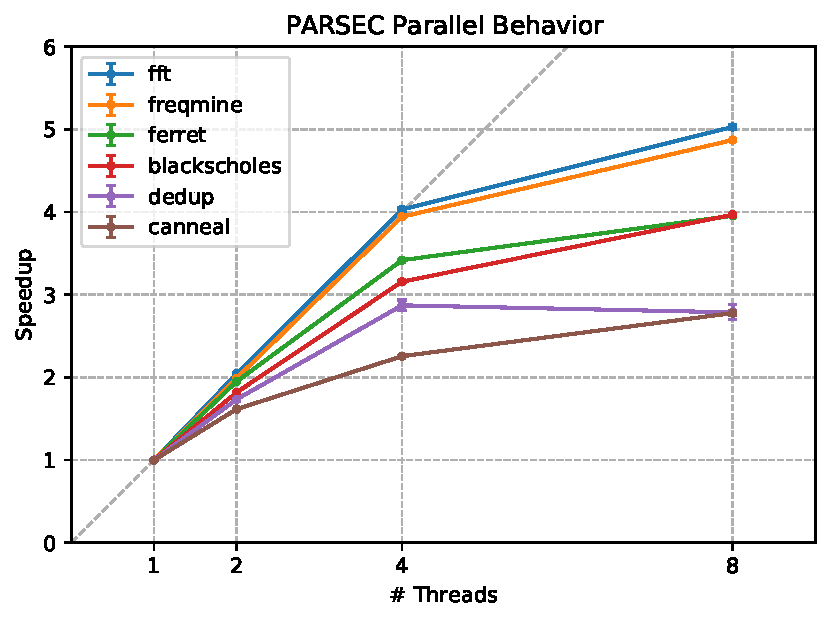
\includegraphics[scale=1]{plot_part2_q3.pdf}}
    \end{center}
    Note: Each experiment was repeated 3 times. We draw the points using the average values and the error bar using the standard deviations. We used the ``real" time for \texttt{blackscholes}, \texttt{canneal}, and \texttt{dedup}. We used the ``QUERY TIME" for \texttt{ferret}. We used the ``Computation Time" for \texttt{fft}. We used the ``FPgrowth cost" for \texttt{freqmine}.
    
\end{enumerate}
\end{document}
